%coagulation verification document
\documentclass[a4paper, 11pt]{article}

\usepackage{amsmath,amssymb,mathrsfs}
\usepackage{graphicx}
\usepackage{fullpage,times}
\usepackage{enumitem}
\usepackage{color}
\usepackage{booktabs,supertabular}
\usepackage{amsthm,thmtools}
\usepackage{xspace}

\theoremstyle{definition}
\newtheorem{defn}{Definition}
\newtheorem{appx}{Approximation}
\newtheorem{assume}{Assumption}
\renewcommand{\listtheoremname}{List of Assumptions and Approximations}

\theoremstyle{remark}
\newtheorem*{rem}{Remark}

% Line spacing
\setlength{\parindent}{0em}
\setlength{\parskip}{1em}

\usepackage[dvipsnames]{xcolor}

%---------
% Draft writing tools
\newcommand{\todo}[1]{\textcolor{red}{\textbf{To-do:\xspace} #1}}
\newcommand{\pbc}[1]{\textcolor{blue}{\textbf{PB comment:\xspace} #1}}
\newcommand{\jjc}[1]{\textcolor{teal}{\textbf{JJ comment:\xspace} #1}}

% Bibliography stuff
\usepackage[sort, numbers]{natbib}
\bibliographystyle{acm}
\setcitestyle{square}

\usepackage{hyperref}

% Hold the serifs, please!
\renewcommand{\familydefault}{\sfdefault}
\usepackage{helvet}

%\usepackage[inline]{../trackchanges}
%\addeditor{Kai}
%\addeditor{Hui}

% Labeling and referencing
\newcommand{\labeleq}[1]{\label{eq:#1}}
\newcommand{\labelsection}[1]{\label{sec:#1}}
\newcommand{\labelsubsection}[1]{\label{subsec:#1}}
\newcommand{\labelappendix}[1]{\label{app:#1}}
\newcommand{\refeq}[1]{Equation~\ref{eq:#1}}
\newcommand{\refsection}[1]{Section~\ref{sec:#1}}
\newcommand{\refsubsection}[1]{Section~\ref{subsec:#1}}
\newcommand{\refappendix}[1]{Appendix~\ref{app:#1}}

% Annotating assumptions(!)
%\newcommand{\assume}{{\bf Assumption: }}

% Math stuff
\renewcommand{\d}[1]{\mathrm{d} #1}
\renewcommand{\vec}[1]{\mathbf{#1}}
\newcommand{\ddt}[1]{\frac{\partial}{\partial t} #1}
\renewcommand{\div}[1]{\nabla \cdot #1}
\newcommand{\dsub}[1]{_{_{#1}}}
\newcommand{\specidx}{L}
\newcommand{\amass}[1]{q\dsub{m,#1,i}}
\newcommand{\vmass}[1]{q\dsub{v,#1}}
\newcommand{\mw}[1]{M\dsub{w,#1}}
% Norm and Absolute value
	\newcommand{\abs}[1]{\left\lvert#1\right\rvert}
	\newcommand{\norm}[1]{\left\lVert#1\right\rVert}	
% derivatives
	\newcommand{\partd}[2]{\frac{\partial #1 }{\partial #2}}
	\newcommand{\partdn}[3]{\frac{\partial^#3 #1}{\partial #2 ^#3}}
	\newcommand{\deriv}[2]{\frac{ d #1}{d #2}}
	\newcommand{\derivn}[3]{\frac{d^#3 #1}{d #2^#3}}	

\begin{document}
\title{Haero Aerosol Model Design Document}
\author{
EAGLES Computation Team\\
}
%\date
\maketitle

% \include puts page breaks after each section, while \input does not.
\chapter{Introduction}
\labelchapter{intro}

Aerosols and aerosol-cloud interactions remain a great source of uncertainty
in global climate models. Haero, the modal aerosol model described in this
document, attempts to help researchers better understand the relevant physical
processes and their contributions to the global climate.

Any model must define abstractions and make assumptions in order to produce
quantitative answers to scientific questions. The abstractions and assumptions
for Haero live in this document. We also describe Haero's software
components---its data structures and programming interface---which are designed
to match these abstractions. In particular, we aim to provide an interface that
allows a scientist to write code that resembles statements made in technical
conversations. We hope that this close correspondence between code and
the related scientific discourse can allow people with different areas of
expertise to contribute to the development of Haero.

In \refchapter{physics}, we very briefly outline the governing equations of
aerosol dynamics from a mathematical perspective. We begin from basic transport
equations formulated in terms of aerosol size distribution functions. We also
describe the assumptions that enter the model at the level of continuous
mathematics (whose approximation errors are present even in analytic
solutions!).

\refchapter{library} introduces the Haero library and its various abstractions.
Because the coupling of aerosol-related processes is still an active area of
research, Haero's software interface focuses on defining specific physical and
mathematical entities, providing a set of elementary building blocks from which
more elaborate models can be constructed.

Next, in \refchapter{testing}, we describe procedures for testing aerosol processes
individually, to make sure they work properly. This type of testing is sometimes
called ``unit testing'' by software people, and ``verification testing'' by
engineers. Either way, it's essential to test your aerosol processes in an
isolated environment with simple inputs that lead to outputs with predictable
characteristics. If you don't test your process this way, {\em you have no idea
what it actually does!}

In \refchapter{processes}, we describe the various processes provided by Haero
that model the stages of the aerosol lifecycle. Here we explain the basic
physical assumptions embedded in each process, along with the details of each
available implementation.

In \refchapter{driver}, we introduce Haero's stand-alone driver program, which
provides a way to run simple aerosol simulations and test parametrizations.
The driver provides a dynamics model to allow researchers to study how transport
and radiative processes affect aerosols.

A comprehensive description of the API appears in \refappendix{api}. The input
specification for the driver is explained in detail in \refappendix{driver_input}.
A glossary of terms and definitions is also provided in \refappendix{glossary}.


\section{Governing Equations}
\labelsection{equations}

Here we offer an extremely abbreviated ``fly-over'' of the evolution equations
that quantify the dynamics of aerosols. Our discussion emphasizes the
mathematical representation of aerosols. For a more detailed explanation of
the underlying ideas, we refer the reader to~\cite{Whitby1991}
and~\cite{Friedlander1977}.

All quantities are in SI units unless specifically mentioned. To keep the
discussion simple and focused, we avoid referencing specific coordinates.

\subsection*{Size Matters}

MAM's approach to modeling aerosols is based on the observations that

\begin{itemize}
  \item the sizes of aerosol particles greatly influence their dynamical
        behavior
  \item these sizes span several orders of magnitude (from 0.001 to 100 microns)
\end{itemize}

Here, a ``particle'' is an individual aerosol molecule with some volume $V_p$.
Aerosol particles consist of polymers, and a particle consisting of a chain of
$i$ monomers is an $i$-mer.

How do we represent a set of aerosol particles in space, given the importance
of their size? In the simplest case (for small $i$-mers), we can denote
$N_i(\vec{x}, t)$ as the number of $i$-mers per cubic meter in the vicinity of
the point $\vec{x}$ at time $t$. In this language, the evolution equation is a
set of coupled advection-diffusion-reaction (ADR) equations acting under the
influence of a bulk velocity $\vec{v}$:

\begin{equation}\labeleq{small_imer_dNdt}
  \ddt{N_i} + \div{(N_i\vec{v})} = \mathcal{D}(\nabla N_i) +
                                   \mathcal{R}(\{N_j\}) +
                                   \mathcal{S}(N_i, t)
\end{equation}

Here we represent terms on the right hand side by

\begin{itemize}
  \item $\mathcal{D}$: terms related to {\it diffusion processes} for $N_i$
  \item $\mathcal{R}$: terms related to {\it reaction processes}, in which
        various $j$-mers combine, react, and dissociate to form particles of
        other types
  \item $\mathcal{S}$: terms related to {\it source and sink processes},
        including external and prescribed sources of $N_i$.
\end{itemize}

We describe the forms of these terms in \refsection{tendencies}. The bulk
velocity $\vec{v}$ is supplied by some dynamical atmospheric model.

For larger $i$-mers ($i > 100$), the above description becomes inadequate, and
we must adopt a description for particle numbers that admits a continuous
number distribution in particle size space.

Let $n(V_p, \vec{x}, t)$ be the number of particles of volume $V_p$ occupying
the point $\vec{x}$ at time $t$. Then the evolution of all $i$-mers is described
by a single ADR equation:

\begin{equation}\labeleq{continuous_dndt}
  \ddt{n} + \div{(n\vec{v})} = \mathcal{D}(\nabla n) +
                               \mathcal{R}(n) +
                               \mathcal{S}(n, t)
\end{equation}

where $\mathcal{D}$, $\mathcal{R}$, and $\mathcal{S}$ have been expressed
in terms of $n$ instead of $N_i$. This is a tidy equation, but $n$ is a
number distribution function that introduces a new dimension---the particle volume
$V_p$---to the solution space. This makes it inconvenient for doing numerical
calculations. In this description, $n$ can assume any shape in particle volume
space, which raises the question of how to constrain the solution in $V_p$.

\subsection*{Moment Equations and the Closure Problem}
We can reduce the size of our solution space by making a few assumptions:

\begin{assume}
  The detailed structure of the number distribution function
        $n(V_p, \vec{x}, t)$ is unimportant to aerosol dynamics.
\end{assume}

If we don't need to obtain the full solution for $n$, we can select a specific
functional form $n(D_p, \vec{x}, t) = n(\vec{x}, t; D_p)$ for it. Then, taking cues from
methods in particle kinetics and turbulence theory, we can integrate the product
of \refeq{continuous_dndt} with powers of $D_p$ to obtain the {\bf moment
equations}

\begin{equation}\labeleq{moments}
  \ddt{\mathcal{M}_k} + \div{(\mathcal{M}_k\vec{v})} = \int_0^{\infty} D_p^k (\mathcal{D} + \mathcal{R} + \mathcal{S}) \d{D_p}
\end{equation}

where $\mathcal{M}_k(\vec{x}, t) = \int_0^{\infty} D_p^k n(\vec{x}, t; D_p) \d{D_p}$
is the ``$k$th moment'' of $n$.

The moment equations are solved by picking a specific form of $n$'s functional
dependence on $D_p$ and playing tricks to avoid actually evaluating the
above integrals. However, the moment equations aren't closed---the advection,
diffusion, reaction, and source terms can all involve $n$ and its spatial
derivatives, and in general, the evolution of $\mathcal{M}_k$ is coupled to higher
moments. To make further progress, we must solve this {\bf closure problem}.

\subsection*{Modal Equations}

Having already given up on obtaining a general solution for $n(\vec{x}, t)$,
we allow ourselves to make another assumption:

\begin{assume}[Modal assumption]
  The number distribution function $n$ is the sum of a set of
        specific number distribution functions $n_i$, each representing a
        {\bf mode} with a specific functional form for a sub-population of
        aerosol particles occupying a certain range in particle size space.
\end{assume}
In other words,

\begin{equation}\labeleq{modal_n}
  n(\vec{x}, t; D_p) = \sum_{i=1}^M n_i(\vec{x}, t; D_p)
\end{equation}

where $n_i$ represents aerosol particles with sizes falling within the range
of mode $i$ and $M$ is the number of modes. Each mode assumes a specific
functional form for $n_i$ in terms of its relevant size as given by $D_p$.
We include the arguments $\vec{x}$ and $t$ to emphasize that this equation holds
at each point in space and at each instant in time for an aerosol system.

\subsubsection*{Log-Normal Distribution Functions}

MAM constructs its multi-modal distribution functions from log-normal
probability distribution functions (PDFs) for each mode $i$. The PDF for mode
$i$ expresses the fraction of aerosol particles present per unit size interval,
in terms of a continuous particle diameter $D_p$ within that mode. Such PDFs
have been found to represent measured aerosol size distributions with a level of
accuracy comparable to that of the relevant measurement
techniques~\cite{Whitby1991}.

\begin{assume}[Log-normal PDF]
The probability distribution function $f_i$ used to construct
        the number distribution function $n_i$ for mode $i$ is a continuous
        function of the particle diameter $D_p$, given as a log-normal distribution,
        \begin{equation}\labeleq{log_normal_pdf}
  f_i(D_p) = \frac{1}{\sqrt{2\pi} D_p \ln \sigma_{g,i}} \ 
      \exp \left [-\frac{(\ln D_p - \ln D_{g,i})^2}{2\ln^2 \sigma_{g,i}} \right]
\end{equation}
where we have introduced the geometric mean $D_{g,i}$ and the geometric standard
deviation $\sigma_{g,i}$ of $D_p$ within mode $i$. 

\end{assume}


In general, these two parameters are determined for each mode via moment equations and corresponding time-evolution equations.
MAM makes an additional simplifying assumption:

\begin{assume}[Constant standard deviation]
  The geometric standard deviation $\sigma_{g,i}>1$ for each mode $i$ is constant in time.  
  The justification for this assumption in \cite{Easter2004,Wilson2001,Whitby1991} is given in \cite{Whitby1981}.
\end{assume}


This PDF can also be expressed in ``logarithmic form'' in terms of $\ln D_p$
of $D_p$:
\begin{equation}\label{eq:log_normal_pdf_log}
  g_i(\ln D_p) = \frac{1}{\sqrt{2\pi} \ln\sigma_{g,i}} \
      \exp \left [ -\frac{(\ln D_p - \ln D_{g,i})^2}{2\ln^2 \sigma_{g,i}} \right]
\end{equation}

Here, $g_i$ is a normal distribution of $\ln D_p$ with a mean of $\ln D_{g,i}$
and standard deviation of $\ln\sigma_{g,i}$.

These PDFs are referred to as {\bf normalized size distribution functions} in
MAM. We can justify this name by multiplying each PDF by the total particle
number density $N_i$ for mode $i$ to obtain the equivalent number distribution
functions:

\begin{align}\label{eq:log_normal_n}
  n_i(D_p) = N_i f_i(D_p) &= \frac{N_i}{\sqrt{2\pi} D_p \ln \sigma_{g,i}} \ 
  \exp \left [ - \frac{(\ln D_p - \ln D_{g,i})^2}{2\ln^2\sigma_{g,i}} \right ] \\
  \hat{n}_{i}(\ln D_p) = N_i g_i(\ln D_p) &= \frac{N_i}{\sqrt{2\pi}\ln \sigma_{g,i}} \ 
	\exp \left [ - \frac{(\ln D_p - \ln D_{g,i})^2}{2\ln^2\sigma_{g,i}} \right ]
\end{align}

\begin{figure}
\centering
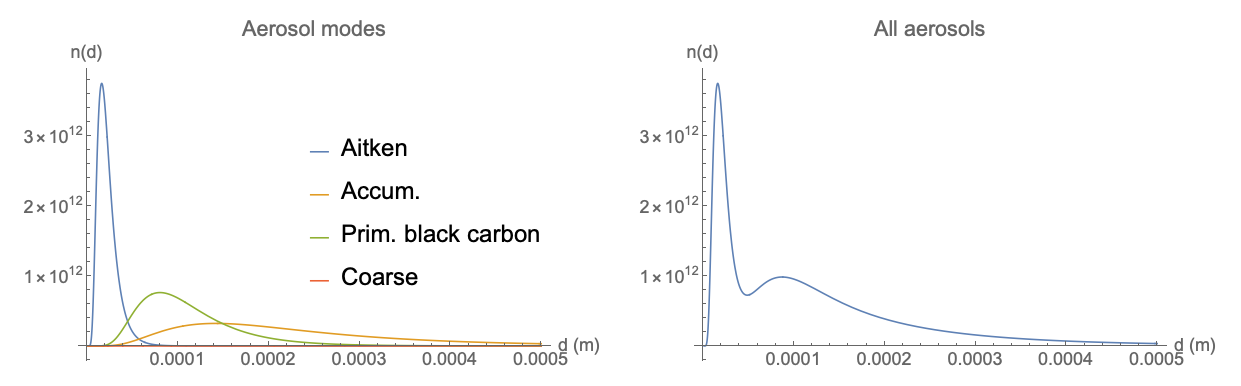
\includegraphics[width=\textwidth]{figures/pdf_examples}
\caption{Normalized size distributions $n_i$ for each mode in the MAM Box Model with $N_i$ set by the \texttt{num\_aer} variable.}\label{fig:mode_dists}  
\end{figure}

The logarithmic form $\hat{n}_i$ is useful because of the relationship
$ n_i(D_p) = \hat{n}_i(\ln D_p)/D_p$, which allows us to write
\begin{equation} \labeleq{equ_norm_lognorm}
  n_i(D_p) \d{D_p} = \hat{n}_i(\ln D_p) \d{\ln D_p}
\end{equation}
to simplify integrands involving number distribution functions.
The benefit of this log-normal functional form choice is that the moment integrals can be defined analytically, obviating the need for potentially costly numerical quadrature \cite[eqns.~(3.7)]{Whitby1991}.
The $k$th moment is given in this case by,
\begin{equation}
  M_k^{(i)} = N_i D_{g,i}^k \exp\left(\frac{k^2}{2}\log^2\sigma_{g,i}\right).
\end{equation}

In particular,
\begin{subequations}
  \begin{align}
    M_0^{(i)} &= \int_0^\infty n_i(D_p)\,d D_p = N_i,\\
    M_1^{(i)} &= \int_0^\infty D_p n_i(D_p)\,d D_p = N_iD_{g,i}\exp({\frac{1}{2}\log^2\sigma_{g,i}}),\\
    M_2^{(i)} &= \int_0^\infty D_p^2n_i(D_p)\,d D_p = N_iD_{g,i}^2\exp(2\log^2\sigma_{g,i}),\\
    M_3^{(i)} &= \int_0^\infty D_p^3n_i(D_p)\,d D_p = N_iD_{g,i}^3\exp(\frac{9}{2}\log^2\sigma_{g,i})
  \end{align}
\end{subequations}


\begin{defn}[Particle size]
  Particle size $\overline{D_i}$ for the $i$th mode is defined by the arithmetic mean diameter associated with the 3rd moment \cite[eqn.~(1)]{Whitby1981}, 
  \begin{equation}
    \overline{D_i} = \left(M_3^{(i)}/N_i)\right)^{1/3} = D_{g,i}\exp\left(\frac{3}{2}\log^2\sigma_{g,i}\right)
  \end{equation}
\end{defn}

\begin{assume}[Particles have spherical shapes] Aerosol particles are spherical, and their size can be parameterized by their diameter $\overline{D_i}$.
The corollaries for area and volume follow, $\overline{A_i} = \pi\overline{D_i}^2$, $\overline{V_i} = \frac{\pi}{6}\overline{D_i}^3$.
\end{assume}
\pbc{I can't make a consistent $\overline{D_i}$ work with more than one $k>0$ moment. Indeed, even \cite[eqn.~(1)]{Whitby1981} notes that this choice must be associated with a specific moment. 
To see this, check: 
$$\overline{D_i}^3 \ne M_3^{(i)}/N_i. $$
The factors multiplying $\log^2\sigma_{g,i}$ do not match.
\\
Perhaps we get away with this incongruity because MAM really only used $M_{0,3}^{(i)}$ and ignores the first and second moments?
}


%\pbc{I've verified the above equations (11), which correspond to \cite[eqns.~(3.7)]{Whitby1991}, but I haven't yet figured out how they relate to $\bar A_i$, $\bar D_i$, and $\bar V_i$, unless: 
%  $$\overline{D_i} = D_{g,i}\exp(\frac{1}{2}\log^2\sigma_{g,i}),~~\overline{A}_i = \pi D_{g,i}^2\exp(2\log^2\sigma_{g,i}),~~ \overline{V_i} = \frac{\pi}{6}D_{g,i}^3\exp(\frac{9}{2}\log^2\sigma_{g,i}).$$
%  In any case, I don't know where the constant exponential factors go.
%  They remain, for example, in \cite[eqn.~(1)]{Whitby1981}.
%}

When we adopt the log-normal assumption, we express our solution for particles in
mode $i$ in terms of its zeroth, first, second, and third moments
$\mathcal{M}_k^{(i)}(\vec{x}, t)$. These are, respectively:
\begin{itemize}
  \item $\mathcal{M}_0^{(i)} = N_i$, the total number of concentration for particles
        in mode $i$
  \item $\mathcal{M}_1^{(i)} = N_i\overline{D}_i$, the number-weighted mean diameter of
        particles in mode $i$
  \item $\mathcal{M}_2^{(i)} = \frac{1}{\pi}N_i\overline{A}_i$, a number-weighted
        surface area of particles in mode $i$
  \item $\mathcal{M}_3^{(i)} = \frac{6}{\pi}N_i\overline{V}_i$, a number-weighted
        volume of particles in mode $i$
\end{itemize}

In this language, the aerosol evolution equation for the $k$th moment of the
$i$th mode is

\begin{equation}\labeleq{modal_evolution}
  \ddt\mathcal{M}_k^{(i)} = F_k^{(i)}(N_i, \overline{D}_i, \overline{A}_i, \overline{V}_i, T, p, \mathsf{...})
\end{equation}

where the air temperature $T$ and the air pressure $p$ enter the moment
equations, via right hand side terms in \refeq{moments}. These are the
{\bf modal equations}.

\begin{assume}
   The time evolution of a moment $\mathcal{M}_k^{(i)}$ can be
    expressed in terms of the quantities $N_i$, $\overline{D}_i$,
    $\overline{A}_i$, $\overline{V}_i$, the air temperature $T$, the pressure $p$, and a few
    selected additional quantities.
\end{assume}

\begin{assume}[2-moment scheme]
  Aerosol dynamics can be represented well by two moments, $M_0^{(i)}$ and $M_3^{(i)}$.
  We therefore need to find equations that describe the time evolution of $M_0^{(i)}$ and $M_3^{(i)}$ in terms of known E3SM variables.
  \begin{itemize}
    \item The number of moles of aerosol per kg of air is $N_i/N_A$, where $N_A$ is the Avogadro Constant.
    \item The mass mixing ratio of aerosol (kg aer.\,/ kg air) is therefore $\displaystyle q^{(i)} = \frac{N_i M_w}{N_A} = \frac{\mathcal{M}_0^{(i)}M_w}{N_A}$, where $M_w$ is the molecular weight (kg/mol) of the aerosol particles in mode $i$.
    \item The mass density of aerosol particles in mode $i$ is therefore, $\rho_{aer}^{(i)} =\rho_{air} \;q^{(i)}$.
    \item The total mass of aerosol particles is then $\displaystyle M_{aer}^{(i)}=\rho_{aer}^{(i)} \overline{V_i} = \frac{\pi}{6}\frac{\rho_{aer}^{(i)}\mathcal{M}_3^{(i)}}{\mathcal{M}_0^{(i)}}$.
  \end{itemize}
\end{assume}

%Solving the closure problem is then reduced to finding expressions for
%$\overline{D}_i$, $\overline{A}_i$, and $\overline{V}_i$ that relate the
%different moments of $n_i$:
%
%\begin{align}
%  \overline{D}_i &= \overline{D}_i(\mathcal{M}_{k_1}^{(i)}/N_i, \mathcal{M}_{k_2}^{(i)}/N_i) \labeleq{D_i}\\
%  \overline{A}_i &= \overline{A}_i(\mathcal{M}_{k_1}^{(i)}/N_i, \mathcal{M}_{k_2}^{(i)}/N_i) \labeleq{A_i}\\
%  \overline{V}_i &= \overline{V}_i(\mathcal{M}_{k_1}^{(i)}/N_i, \mathcal{M}_{k_2}^{(i)}/N_i) \labeleq{V_i}
%\end{align}
%
%Here, we formulate the above expressions by the selecting pairs of moments that
%contribute to the evolution of each quantity for mode $i$.
%
%\begin{assume}[Moment pairs]
% The averaged quantities $\overline{D}_i$, $\overline{A}_i$,
%    and $\overline{V}_i$ can each be expressed as a function of a pair of
%    specific number-normalized moments for the $i$th mode.
%\end{assume}

\subsubsection*{Mode definitions in MAM4}

The choices of size range and width for the modes in MAM are based on
measurements of tropospheric aerosols (see~\cite{Easter2004} and references therein).
Table~\ref{tab:mode_size_parameters} shows the relevant parameters for MAM4,
the 4-mode legacy MAM model.

%------------------- table: mode parameters ---------------
\begin{table}[htbp]
\centering
%\caption{
%Geometric mean dry diameter ($D\dsub{gn,d,i}$, unit:
%$\rm \mu m$) and geometric standard deviation ($\sigma\dsub{g,i}$)
%of the number size distribution of each log-normal mode.
%}
%\begin{tabular}{ccccc}
%  \toprule
%  Mode        &  Lower bound of $D\dsub{gn,d,i}$  &  $D\dsub{gn,d,i}$   &
%  Upper bound of $D\dsub{gn,d,i}$  &  $\sigma\dsub{g,i}$ \\
%  \midrule
%  Aitken 	            &  0.0087  &   0.026   &   0.052  &  1.6 \\
%  Accumulation     &  0.0535  &   0.11      &   0.44    &  1.8 \\
%  Coarse               &  1.0        &   2.0       &   4.0      &  1.8 \\
%  Primary carbon  &  0.01      &   0.05      &   0.1      &  1.6 \\
%  \bottomrule
%\end{tabular}
\caption{Parameters of log-normal modes in MAM4.}
\label{tab:mode_size_parameters}
\begin{tabular}{cccccc}
  \toprule
  Mode           &  Lower bound of $D\dsub{gn,d,i}$
                 &  Upper bound of $D\dsub{gn,d,i}$  &  $\sigma\dsub{g,i}$ 
                 & $N_i(0)$\\
  \midrule
  Aitken 	 &  0.0087  &   0.052  &  1.6     & 7.9031E7\\
  Accumulation   &  0.0535  &   0.44   &  1.8 & 7.9697E7\\
  Coarse         &  1.0     &   4.0    &  1.8 & 8.0361E7\\
  Primary carbon &  0.01    &   0.1    &  1.6 & 8.1022E7\\
  \bottomrule
\end{tabular}
\end{table}
%-------------

Thus, in MAM, all modes have the same mathematical form, but the parameters
are different for each mode.

\subsection*{Multi-Species Modes}

We have derived the modal equations assuming that each mode contains a
population of undifferentiated aerosol particles. 
We assume that each particle is composed of several, potentially different, chemical species, which corresponds to the following assumption.
%If we wish to track individual
%particle species within a mode, we may do so by expressing the population of a
%mode as the sum of its constituent species in the modal assumption, adding
%a species index $s$ to the number distribution function $n$:
%
%\begin{equation}\labeleq{modal_multi_species}
%  n(\vec{x}, t; D_p) = \sum_{i=1}^M \sum_{s=1}^S n_{i,s}(\vec{x}, t; D_p)
%\end{equation}
%
%with $S$ as the number of species. Then we can carry out the subsequent analysis
%as before, breaking up the moments into species-specific parts
%$\mathcal{M}_k^{(i,s)}$ and expressing the total $k$th moment as the sum of these
%parts:
%
%\begin{equation}
%  \mathcal{M}_k^{(i)} = \sum_{s=1}^S \mathcal{M}_k^{(i,s)}
%\end{equation}
%
%Then the multi-species modal evolution equations are
%
%\begin{equation}\labeleq{modal_multi_species_evolution}
%  \ddt\mathcal{M}_k^{(i,s)} = F_k^{(i,s)}(N_{i,s}, \overline{D}_{i,s}, \overline{A}_{i,s}, \overline{V}_{i,s}, T, p, \mathsf{...})
%\end{equation}
%
%with species-specific equivalents of the quantities in \refeq{modal_evolution}.

\begin{assume}[Internally mixed]
  All aerosol species within a mode are assumed to be carried uniformly by all particles represented by the mode's log-normal distribution function, i.e., within each mode, particles are internally mixed.
\end{assume}

\begin{assume}[Additive particle volume]
  Quantitatively, the internal mixing assumption implies that the volume of each individual particle is the sum of the volumes of its various constituents; in this case, the species within the mode.  
\end{assume}


These assumption has several implications:
\begin{enumerate}
  \item All species within mode $i$ share the same particle size distribution; as a corollary, they also share the same number concentration,
  \begin{equation}
    N_{i,q} = M_0^{(i)} = N_i,
  \end{equation}
  for all species $q$ in mode $i$.
\end{enumerate}

\section{Modes, Species, and Chemical Reactions}
\labelsection{modes_and_species}

In this section, we introduce data types in Haero that are used to define a
physical system involving aerosols. These data types don't hold state
information---they only specify the modes and species present in a system,
and the chemical reactions that affect their populations.

Haero is written primarily in C++, so we describe C++ data structures in
this section. However, Haero also provides a Fortran interface that can be
used by scientists to develop and test new parametrizations. Both the C++
and Fortran application programming interfaces (APIs) are described in
detail in \refappendix{api}.

\subsection{The Mode Data Type}\labelsection{mode_data_type}

We've seen how the dynamics of aerosols can be represented mathematically
by evolution equations for moments of modal distribution functions. Modes
simplify the description of aerosol particles in terms of their size: instead of
representing a population of particles with a distribution function
$n(V_p, \vec{x}, t)$ that varies continuously with the size of the particle, we
introduced $M$ discrete modes and declared that these modes partition the
population of aerosol particles in the sense of the modal assumption as given
by \refeq{modal_n}.

The essential information in a mode is the range of particle sizes it
encompasses, $[D_{\min}, D_{\max}]$, and its geometric standard deviation,
$\sigma_g$. In Haero's C and C++ interfaces,
we represent an aerosol mode with the \verb|Mode| struct:

\begin{verbatim}
struct Mode {
  std::string name;  // a unique identifier for the mode
  Real min_diameter; // the mode's minimum particle diameter
  Real max_diameter; // the mode's maximum particle diameter
  Real mean_std_dev; // the geometric mean standard deviation for the mode
}
\end{verbatim}

In principle, a Haero calculation can support any number of modes, but care
must be taken to ensure that the modal assumptions remain valid, and that
the parametrizations selected can accommodate the given modes.

\subsection{The Species Data Type}\labelsection{species_data_type}

{\bf WARNING: This section is under construction!}

Each aerosol mode consists of one or more particle species. Additionally,
gas particles also come in different species. Both aerosol particles and
gas particles have physical properties that are described by the
\verb Species  data type.

A particle species is a specifically-identified molecular assembly with
a number of relevant physical properties. The fundamental description of a
species includes

\begin{itemize}
  \item a symbolic name (e.g. \verb SO4 , for sulfate)
  \item a descriptive name (e.g. \verb "sulfate" )
  \item its elemental composition (how many atoms of each type it possesses)
  \item its net electrical charge (in units of the elementary charge $|e|$)
\end{itemize}

We represent this information in the following way:

\begin{verbatim}
struct Species {
  std::string name;                       // full species name
  std::string symbol;                     // abbreviated symbolic name
  std::map<std::string, int> composition; // elemental make-up of species
  int charge;                             // net electrical charge
};
\end{verbatim}

The \verb composition  field in the \verb Species  struct maps the name of
a chemical element to the number of atoms of that type that appear within
the species.

\subsection{Chemistry Data Types}\labelsection{chem_data_types}

TBD: we currently don't have a candidate for a chemical mechanism, though
we are considering Cantera.


\section{Simulation Contexts}
\labelsection{contexts}

\subsection{Uniform atmosphere}

This is the simplest possible simulation setting, with each level of a physics column containing the exact same environment.  
It provides a means of testing aerosol-specific methods in isolation.

\subsection{Single-column}

In this setting, we use a one-dimensional (vertical) atmosphere and tests of increasing complexity.
The simplest conditions are a  statically stable, hydrostatically balanced atmosphere, with vertical velocity $w=0$.
We assume a linear temperature profile with constant lapse rate $\Gamma = -\partial T/\partial z$,
\begin{equation}
  T(z) = T_0 - \Gamma z,
\end{equation}
where $T_0$ is the reference temperature at $z=0$ (K).  
Note that the atmosphere is statically stable if $\Gamma < \Gamma_{dry}$, where $\Gamma_{dry}$ is the dry adiabatic lapse rate, $\Gamma_{dry} = 0.0098$ K/m and that an isothermal atmosphere is defined by $\Gamma = 0$.
Using the ideal gas law, $p = \rho R T$ and the hydrostatic equation $\partial p/\partial z = -\rho g$, we derive the relations between pressure and height,
\begin{equation}
  p(z) = \begin{cases}
          p_0\exp\left(\frac{-g z}{RT_0}\right) & \Gamma = 0,\\[0.5em]
          p_0\, T_0^{-g/(R\Gamma)}\left(T_0 - \Gamma z\right)^{g/(R\Gamma)} & \Gamma \ne 0,
        \end{cases}
\end{equation}
\begin{equation}
  z(p) = \begin{cases}
         -\frac{R T_0}{g}\log\frac{p}{p_0} & \Gamma = 0,\\[0.5em]
         \frac{T_0}{\Gamma}\left(1 - \left(\frac{p}{p_0}\right)^{R\Gamma/g}\right) & \Gamma \ne 0,
       \end{cases}
\end{equation}
where $p_0$ is the reference pressure at $z=0$ and $T=T_0$.

%A nonzero vertical velocity may be prescribed using a simple analytic function, such as
%\begin{equation}
%  w(z,t) = w_0\cos\left(\frac{2\pi t}{W_P}\right)\sin\left(\frac{2\pi z}{z_{top}}\right),
%\end{equation}
%where $w_0$ is the maximum vertical velocity (m/s), $W_P$ is the velocity period in seconds, and $z_{top}$ is the top of the model (m).
%Note that this velocity has nonzero divergence, $\partial w/\partial z \ne 0$.
%
%\pbc{This velocity probably destroys hydrostatic balance, without similar adjustments to pressure.}

As in \cite{Taylor2020}, we use a pressure-based vertical mass coordinate defined by the arbitrary variable $s$ and the hydrostatic pressure $\pi$ so that $s=0$ at $z=z_{top},~p= p_{top}$ and $s=1$ at $z=0,~p=p_0$.
The column is discretized by $n_{lev}$ vertical levels; pressure is defined at each level, while the height $z$ (or the geopotential $\phi=gz$) is defined at the $n_{lev}+1$ level interfaces (note that both the model top and the surface are interfaces).
Transported quantities such as water vapor and aerosols are defined at level midpoints; the thermodynamic variable ($T$, potential temperature $\theta$, or virtual potential temperature $\theta_v$) are also defined at level midpoints.
Vertical velocity and hydrostatic pressure are defined at interfaces; see \cite{Taylor2020} for details.


\subsubsection{Single column dynamics}

We define dynamics by the vertically Lagrangian form of the HOMME $\theta$-model \cite{Taylor2020}, using the vertical direction only,
\begin{subequations}\label{eq:column_dynamics}
  \begin{align}
    \deriv{w}{t} &= -g(1-\mu),\\
    \deriv{\phi}{t} &= gw, \\
    \deriv{\Theta}{t} &= 0, \\
    \deriv{\partd{\pi}{s}}{t} &= 0,\\
    \deriv{q_v}{t} &= 0,     
  \end{align}
where $\partd{\pi}{s}$ is the pseudo-density, $\mu$ is the ratio of pressure to hydrostatic pressure, $\mu = \partd{p}{s}/\partd{\pi}{s}$. 
In hydrostatic conditions, $\mu \equiv 1$.
The water vapor mixing ratio is $q_v$.
The conservative form of potential temperature $\Theta = \partd{\pi}{s}\theta_v$, where $\theta_v$ is the virtual potential temperature, is related by the equation of state to the geopotential $\phi$,
\begin{equation}
  \partd{\pi}{s} = -R\Theta \frac{\Pi}{p},
\end{equation}
where $\Pi$ is the Exner function,
\begin{equation}
  \Pi =\left(\frac{p}{p_0}\right)^{R/c_p}.%= \left(\frac{R_d}{p_0}\rho\theta_v\right)^{R_d/c_p}
\end{equation}
\end{subequations}
\pbc{Check: 6 equations, 6 unknowns: $w, \phi, \partd{\pi}{s}, q_v, \theta_v, p$.}
For our purposes, it suffices to approximate $\theta_v = \theta(1+0.61q_v)$ as in \cite{KlempWilhelmson1978}, where the potential temperature $\theta = T(p_0/p)^{\kappa}$, with the dry-air constant $\kappa = R_{dry}/c_p$.

Srivastava \cite{Srivastava1967} present a simple model of a one-dimensional cumulus cloud based on warm rain microphysics.
\pbc{Rogers \& Yau provide a better summary; it's 1D Euler plus Kessler microphysics.}
Moisture is represented by $q_v,~q_c,$ and $q_r$, the mixing ratios of water vapor, cloud water droplets, and rain water droplets, respectively.
The model was developed to show the effects of momentum transfer from falling rain on the cloud's vertical velocity; here, we adapt to test various aerosol-related parameterizations.
The column is initially defined by statically unstable hydrostatic balance, with lapse rate $\Gamma = 0.0068$ K/m.
We assume a constant background state with pressure $\overline{p}(z)$, density $\overline{\rho}(z)$ and temperature defined by $\overline{T}(z) = T_0 - \Gamma z$ and hydrostatic balance.
The perturbation temperature $T' = T - \overline{T}(z)$.
The model equations are:
\begin{subequations}
  \begin{align}
    \partd{w}{t} + w\partd{w}{z} & = g\left( \frac{T'}{T} - (q_c + q_r)\right),\\
    \partd{q_v}{t} + w\partd{q_v}{z} &= E_1 + E_2, \\
    \partd{q_c}{t} + w\partd{q_c}{z} &= E_1 - P, \\
    \partd{q_r}{t} + w\partd{q_r}{z} &= - q_r\partd{w_r}{z} - w_r\partd{q_r}{z} - \frac{q_r w_r}{\overline{\rho}}\partdn{\overline{p}}{z}{2}  - E_2 + P,\\
    \partd{T}{t} + w\partd{T}{z} &= -w\Gamma - \frac{L}{c_p}(E_1+E_2),
  \end{align}
\end{subequations}
where $E_1$ describes evaporation and condensation of vapor-to-cloud water, $P$ is the rain water production term that accounts for autoconversion and accretion, $w_r \le 0$ is the rain fall velocity, $L$ is the latent heat of evaporation, and $c_p$ is the specific heat (at constant pressure) of air.

The evaporation rate depends on the saturation of the air,
\begin{equation}
  E_1 = a_0\left(\frac{q_v}{q_{vsat}} - 1\right),
\end{equation}
where $q_{vsat}$ is the saturation mixing ratio given by the Tetens equation,
\begin{equation}
  q_{vsat}(T) = \frac{380.042}{\overline{p}}\exp\left(17.27 \frac{T-273}{T-36}\right).
\end{equation}

%Cloud water in \cite{Srivastava1967} is generated simply,
%\begin{equation*}
%  P_c = -w\partd{q_v}{z};
%\end{equation*}
%we add terms to represent cloud water droplet activation via condensation nuclei,
%\begin{equation}\label{eq:qc_prod}
%  P_c = -w\partd{q_v}{z} + A(T, \Delta T, q_v,q_{aer}),
%\end{equation}
%where $q_{aer}$ is the mixing ratio of aerosol cloud condensation nuclei.
%\todo{Need some help with \eqref{eq:qc_prod}.}
%Rain production is decomposed into three subprocesses, $P_r=P_1 + P_2 + P_3$.
%The first subprocess represents evaporation in convective downdrafts,
%\begin{equation}
%  P_1 = -\mu(w) w \partd{q_v}{z}, \quad \mu(w) = \begin{cases} 1 & w<0, \\ 0 & w >= 0\end{cases}.
%\end{equation}
%The second subprocess represents cloud water conversion,
%\begin{equation}
%  P_2 = \begin{cases} 0 & q_c \le  q_c^{(crit)} \\ \alpha(q_c - q_c^{(crit)}) & q_c >  q_c^{(crit)}\end{cases},
%\end{equation}
%where $\alpha$ is a constant parameter representing the conversion time scale and $q_c^{(crit)}$ is an additional parameter, representing the critical value of cloud water, above which cloud water is converted to rain water.
%\pbc{Perhaps we should consider smoothing out these piecewise functions?}
%The last subprocess represents accretion, the capture of cloud drops by rain drops,
%\pbc{I assume that conversion implies $C: q_c,q_c \mapsto q_r$, whereas accretion implies $Ac:q_c,q_r\mapsto q_r$.}
%The model assumes that rainwater fall speed is proportional to droplet size, $W_r(D) = a D^b$, where $a$ and $b$ are constants, and that rain water droplet sizes are governed by the distribution function $N(D) = N_0e^{-\lambda} D$, where $\lambda = 3.67/D_0$ is a variable parameter related to $D_0$, the median diameter of rainwater droplets \cite[eqn.~(18)]{Srivastava1967}.
%With these assumptions, the expression for accretion is
%\begin{equation}
%  P_3 = \frac{\pi N_0 a \rho \Gamma(3+b) q_r}{4\lambda^{3+b}},
%\end{equation}
%where $\Gamma$ represents the Gamma Function (not a lapse rate).
%The same assumptions give the expression for rain fall velocity,
%\begin{equation}
%  w_r = \frac{a\Gamma(4+b)}{6\lambda^b}.
%\end{equation}

Initial conditions for $w$ and $q_c$ are defined by solving the above equations with $q_r=0$, and $w(z_c)=q_c(z_c) = 0$, $T(z_c) = 277$ K, where $z_c$ is the height of the cloud base.
\todo{Have to figure these out ourselves. Using standard thermodynamics and hydrostatic balance.}
\pbc{I believe cloud base is the first point above $z=0$ where $q_c>0$.}
The bottom boundary condition is $w(0) = 0$.
At $z_{top} = 9.5$ km, if $w(z_top)>0$ then the equations are solved without regard for the boundary; if $w(z_top)<=0$ the other variables are held constant.

%------------------- table: cloud model parameters ---------------
\begin{table}[htbp]
\centering
\caption{Parameters of the 1D cloud model.}
\label{tab:cloud_model_parameters}
\begin{tabular}{ccccc}
  \toprule
  Parameter      &  value 1
                 &  value 2
                 & value 3\\
  \midrule
  $a$ 	 &  1500 cm$^{1/2}$/s  &  --  & -- \\
  $b$    &  0.5                &  --  & --  \\
  $\lambda$  &  1.0            &  --  & --  \\
  $N_0$ &  80 (gm cm)$^{-1}$   &  --  & --  \\
  $\alpha$ & 2.0E-5 s$^{-1}$ (14 hr) & 4.0E-5 s$^{-1}$ (7 hr) & 4.0E-5 s$^{-1}$ (4 min) \\
  $q_c^{(crit)}$ & 0 & 3 gm/kg & 3 gm/kg \\
  \bottomrule
\end{tabular}
\end{table}
%-------------



\subsection{Embedded parameterization}
\section{Tendencies and Coupling Terms}
\labelsection{tendencies}



\appendix
\chapter{Glossary}
\labelappendix{glossary}

This section contains definitions of important terms and mathematical quantities
used in Haero.

\section{Terminology}
\labelappendixsection{terminology}

\begin{itemize}
  \item Cloud Condensation Nuclei (CCN):
  \item Precursors:
  \item Secondary Aerosols:
\end{itemize}

\section{Mathematical Notation}
\labelappendixsection{notation}

The following symbols are used in equations within Haero's aerosol processes.
Relevant units are given in square brackets next to their symbols. [-] indicates
that a quantity is unitless.

\begin{itemize}
  \item $T$ [K]: air temperature

  \item $p$ [Pa]: air pressure

  \item $\specidx$: index of chemical species

  \item $\mw{\specidx}$ [kg/kmol]: molecular weight of species $\specidx$

  \item $\mathscr{R}$ [J/kmol/K]: universal gas constant

  \item $R_{\specidx}$ [J/kg/K]: gas constant specific to species $\specidx$:
        $R_{\specidx} = \mathscr{R}/\mw{\specidx}$

  \item $c\dsub{air}$ [kmol air / m$^3$ air]: molar concentration of dry air:
    \begin{equation}
      c\dsub{air} = \frac{p}{\mathscr{R}T} = \frac{\rho\dsub{air}}{M\dsub{air}}
    \end{equation}
    where $\rho\dsub{air}$ and $M\dsub{air}$ are the density and molecular weight
    of dry air, respectively. Note that
    $M\dsub{air} = 28.966$~kg~$\cdot$~kmol$^{-1}$ in E3SM.

  \item $\rho\dsub{\specidx}$ [kg/m$^3$]: density of species $\specidx$
        (gas, liquid or solid)
    \hwc{For liquid- and solid-phase species there seems to be two types of
      densities:
      \begin{enumerate}
        \item mass divided by the volume of air in which they are suspended
        \item mass divided by the volume the liquid or solid matter occupies
      \end{enumerate}
      $\rho\dsub{\specidx}$ seems to be fall in to the first type. Let's watch
      out for places of potential confusion.}

  \item $i$, $j$: indices of log-normal modes

  \item $I$: total number of log-normal modes

  \item $D\dsub{p}$: particle diameter, unit: $\rm m$

  \hwc{Which of the following notations need to be distinguished for
       interstitial and cloud-born aerosols?}
  \jsc{We at least need different notations for interstitial and cloud-borne
       aerosols for $\amass{\specidx}$ and $q\dsub{n,i}$ in the rename process.
       All the other parameters are related to $\amass{\specidx}$ and
       $q\dsub{n,i}$ so we may also need to use different notation.}

  \item $N\dsub{i}$ [\#/m$^{-3}$]: number concentration of particles in mode $i$

  \item $n\dsub{i} (D\dsub{p})$ [m$^{-4}$]: size distribution of aerosol
        particles in mode $i$, expressed as a function of $D\dsub{p}$
        (\refeq{n_Dp})

  \item $n\dsub{i} (\ln D\dsub{p})$ [m$^{-3}$]: size distribution of aerosol
        particles in mode $i$, expressed as a function of $\ln D\dsub{p}$
        (\refeq{n_lnDp})

  \item $n\dsub{norm,i} (\ln D\dsub{p})$ [-]: $n\dsub{i} (\ln D\dsub{p})$
        normalized by the mode's number concentration $N\dsub{i}$

  \item $D\dsub{gn,d,i}$ [m]: geometric mean of dry particle diameter
        $D\dsub{p}$ in mode $i$

  \item $D\dsub{gn,w,i}$ [m]: geometric mean of wet particle diameter
        $D\dsub{p}$ in mode $i$

  \item $\sigma\dsub{g,i}$ [-]: geometric standard deviation of $D\dsub{p}$ in
        mode $i$
        \hwc{Why is it unitless?}
        \jsc{The unit of $\sigma\dsub{g,i}$ should be the same as that of
             $D\dsub{p}$. $\ln D\dsub{p}$ and $\ln \sigma\dsub{g,i}$ are
             unitless. According to Seinfeld's book, when we write
             $\ln D\dsub{p}$ and $\ln \sigma\dsub{g,i}$, we really mean
             $\ln \frac{D\dsub{p}}{1}$ and $\ln \frac{\sigma\dsub{g,i}}{1}$,
             where 1 is the ``reference'' particle diameter or standard
             deviation and not explicitly indicated.}

  \item $V\dsub{d,i}$ [m$^3$ particles/m$^3$ dry air]: volume concentration of
        dry aerosol particles in mode $i$

  \item $V\dsub{w,i}$ [m$^3$ particles/m$^3$ dry air]: volume concentration of
        wet aerosol particles in mode $i$

  \item $V\dsub{\specidx,i}$ [m$^3$ species $\specidx$/m$^3$ dry air]: dry
        volume of species $\specidx$ in mode $i$

  \item $q\dsub{n,i}$ [\#/kmol]: total number mixing ratio of particles in mode
        $i$

  \item $\amass{\specidx}$ [kmol species $\specidx$/kmol dry air] in microphysics,
        [kg species $\specidx$/kg dry air] in dry/wet deposition: mass mixing
        ratio for aerosol species $\specidx$ in mode $i$
        % listed in Section~\ref{sec:MAM_procs_and_eqns})

  \item $\rho\dsub{d,i}$ [kg dry aerosol particles/m$^3$ dry aerosol particles]:
        density of dry aerosol particles in mode $i$

  \item $\rho\dsub{w,i}$ [kg of wet aerosol particles/m$^3$ wet aerosol
        particles]: density of wet aerosol particles in mode $i$

  \item $\vmass{\specidx}$ [kmol species $\specidx$/kmol dry air] in microphysics,
        [kg species $\specidx$/kg dry air] in other parameterizations: mass
        mixing ratio for gas species (vapor)

  \item $\Delta t\dsub{phys}$ [s]: time step size for aerosol physics
\end{itemize}

\section{The MAM Application Programming Interface}
\labelappendix{api}


\section{Driver Input Specification}
\labelsection{input}

Below is the input specification for the Haero driver. The spec uses
[YAML](https://yaml.org/). Compared to Fortran namelists, YAML offers

\begin{itemize}
  \item {\bf better readability}: YAML files are flexible, and don't have a lot
    of "kibble" (braces, tags, and other stuff you see routinely in fancier
    markup like XML, HTML, and so on). They're very easy to read.
  \item {\bf better validation}: YAML files have named entries that can be
    used or ignored, depending on the needs of the particular application.
    Also, the file format allows for error checking.
  \item {\bf better language support}: Fortran namelists are so-called because
    they are only available to Fortran. YAML has libraries that allows it to
    be used with several programming languages (including Fortran!). This makes
    it easier for tools and other applications to use similar input files. In
    particular, this allows workflows to use a single input file to define a
    workload that can be processed with several tools.
  \item {\bf support for lists and maps}: YAML offers constructions for
    dynamically-sized datasets. As we move MAM toward runtime configurability,
    the ability to add species (and perhaps even modes) to an input file
    becomes more important.
  \item {\bf a larger support community}: Fortran remains a niche language,
    which often instills a sense of pride in scientists. Unfortunately, the
    downside to belonging to a small community of specialists is that the tools
    are invariably of lower quality than more commonly-used tools. One needs
    only to witness the notorious ongoing issues with Fortran compilers to see
    this phenomenon firsthand.
\end{itemize}

This specification is for use only with the Haero driver. The library provides
no input/output interface---it assumes that the model in which it's embedded
does the work of assembling input data and loading it into the appropriate
data structures.

The Haero driver is a single-column aerosol dynamics simulator---it doesn not
model horizontal dynamics. However, depending on how initial conditions are
specified, it's possible to generate ensembles whose members are individual
atmospheric columns. Because the columns are independent of one another, these
ensembles can be run entirely within a single simulation, allowing the driver
to take advantage of parallelism, and allowing statistics and measures of
convergence to be generated.

\subsection*{Sections}

A YAML file consists of several named sections. Each of these sections can
contain data and metadata. Sections are a powerful tool for organizing input
using simple concepts with human-readable notation.

\subsubsection*{Modes}

The \verb modes  section defines the particle size modes available to a MAM
model. As we discussed in \refsection{modes_and_species}, a mode has metadata
specifying its size range and its geometric standard deviation.

\begin{verbatim}
modes:
  aitken:
    D_min: 0.0087
    D_max: 0.052
    sigma: 1.6
  accumulation:
    D_min: 0.0535
    D_max: 0.44
    sigma: 1.8
  coarse:
    D_min: 1.0
    D_max: 4.0
    sigma: 1.8
  primary_carbon:
    D_min: 0.01
    D_max: 0.1
    sigma: 1.6
\end{verbatim}

Particle diameters and $\sigma$ are measured in $\mu\mathrm{m}$.

The \verb modes  section is essentially a map whose keys are mode names
(\verb aitken , \verb accumulation , \verb coarse , and \verb primary_carbon ,
in the example above), and whose values are themselves maps. The map for a given
mode contains the following fields:

\begin{itemize}
  \item \verb D_min : the minimum diameter of particles belonging to the mode
  \item \verb D_max : the maximum diameter of particles belonging to the mode
  \item \verb sigma : the geometric mean standard deviation for the size
                      distribution for particles belonging to the mode
\end{itemize}

Everything in a mode must be completely specified---there are no default values.

\subsubsection*{Aerosol Species}

Aerosol species populate each of the defined modes, and are defined in the
\verb aerosols  section. As we discussed in \refsection{modes_and_species}, a
species is defined by its elemental composition and its electric charge (given
in units of the electronic charge $|e|$).
%The \verb species  section follows the same format as defined by
%\href{https://cantera.org/documentation/dev/sphinx/html/yaml/species.html}{Cantera}.

Like the \verb modes  section, the \verb aerosols  section is a map whose keys
are {\em symbolic names} of aerosol particle species (e.g. \verb SO4  for
sulfate particles):

\begin{verbatim}
aerosols:
  SO4:
    name: sulfate
  NH4:
    name: ammonium
  POA:
    name: primary organic aerosol
  SOA:
    name: secondary organic aerosol
  BC:
    name: black carbon
  SS:
    name: sea salt
  DST:
    name: dust
  MOA:
    name: marine organic aerosol
\end{verbatim}

An aerosol species has the following fields:

\begin{itemize}
  \item \verb name : the full name for the species (e.g. \verb sulfate  for
    \verb SO4 ). You don't need to quote the full name, even if
                     it contains spaces.
\end{itemize}

\subsubsection*{Gas Species}

Gas species exist in the atmosphere, and aren't associated with modes. These
species are defined in the \verb gases  section.

The \verb gases  section is identical in structure to the
\verb aerosols section:

\begin{verbatim}
gases:
  SO2:
    name: sulfur dioxide
  H2SO4:
    name: sulfuric acid
  SOAG:
    name: single semi-volatile organic gas-phase species
  NH3:
    name: ammonia
\end{verbatim}

A gas species has the following fields:

\begin{itemize}
  \item \verb name : the full name for a gas species (e.g.
                     {\verb sulfur dioxide} for \verb SO4 . You don't need to quote the
                     full name, even if it contains spaces.
\end{itemize}

\subsubsection*{Physics}

In this section, we tell the Haero driver what physical processes we wish
to simulate. Every field in this section assumes a \verb true  or
\verb false  value, so it's really just a set of ON/OFF switches. Valid fields
are:

\begin{itemize}
  \item \verb growth : enables particle growth modeling
  \item \verb gas_chemistry : enables the gas chemistry mechanism
  \item \verb cloud_chemistry : enables the cloud chemistry mechanism
  \item \verb gas_aerosol_exchange : enables exchange processes that occur
                                     between gas and aerosol particles
  \item \verb mode_transfer : enables the transferring particles between modes
  \item \verb nucleation : enables aerosol particle formation processes
  \item \verb coagulation : enables inelastic aerosol collision processes
\end{itemize}

\subsubsection*{Grid Parameters}

This section contains information about the computational grid used by the
Haero driver.

\begin{verbatim}
grid:
  num_columns: 1
  num_levels:  72
\end{verbatim}

There are two required fields:

\begin{itemize}
  \item \verb num_columns : the number of independent atmospheric columns
  \item \verb num_levels : the numer of vertical cells in each column
\end{itemize}

\subsubsection*{Atmospheric Conditions}

In each cell within each column, there exist atmospheric conditions that
provide important parameters---temperature, pressure, relative humidity, etc---
that govern physical processes. The \verb atmosphere  section allows you
to specify one of a handful of simple models for obtaining those parameters.
Each model has its own parameters.

First and foremost, you specify a model with the \verb model  field within
the \verb atmosphere  section. Supported models are:

\begin{itemize}
  \item \verb uniform : a simple atmospheric environment in which columns are
                        assumed to be short in comparison to the height of the
                        atmosphere so that all conditions are uniform
  \item \verb hydrostatic : an atmospheric environment in hydrostatic
                            equilibrium, with the relationship between pressure
                            and temperature defined by an ideal gas law
\end{itemize}

These models are described in detail in \refsection{contexts}. Here we simply
list valid fields for each model. These fields are specified alongside the
\verb model  field in the \verb atmosphere  section. Tables~\ref{tab:uniform_atm}
and~\ref{tab:hydrostatic_atm} list fields for the \verb uniform  and
\verb hydrostatic  models.

\begin{table}[htbp]
\caption{Uniform atmosphere parameters}
\centering
\label{tab:uniform_atm}
\begin{tabular}{ccc}
  \toprule
  Parameter   & Description                  & Units   \\
  \midrule
  \verb mu    & Mean molecular weight of air & kg/mol  \\
  \verb H     & Scaled atmospheric height    & m       \\
  \verb p0    & Pressure                     & Pa      \\
  \verb T0    & Temperature                  & K       \\
  \verb phi0  & Relative humidity            & -       \\
  \verb N0    & Cloud fraction               & -       \\
  \bottomrule
\end{tabular}
\end{table}

\begin{table}[htbp]
\caption{Hydrostatic atmosphere parameters}
\centering
\label{tab:hydrostatic_atm}
\begin{tabular}{ccc}
  \toprule
  Parameter   & Description                  & Units   \\
  \midrule
  \verb mu    & Mean molecular weight of air & kg/mol  \\
  \verb H     & Scaled atmospheric height    & m       \\
  \verb p0    & Pressure                     & Pa      \\
  \verb T0    & Temperature                  & K       \\
  \verb phi0  & Relative humidity            & -       \\
  \verb N0    & Cloud fraction               & -       \\
  \bottomrule
\end{tabular}
\end{table}

\subsubsection*{Initial Conditions}

The \verb initial_conditions section defines the initial state of an aerosol
system. There are subsections for \verb aerosols , for \verb gases , and
for \verb modes  themselves.

In the Haero driver, the initial state for an aerosol species is specified by
its modal mass fractions, given for every mode occupied by that species. The
nodal mass fraction of an aerosol species is the fraction of the total mass of
the mode's particles occupied by that species.

Meanwhile, the initial state for a gas is its mole fraction---the number of
moles of gas per mole of air.

Finally, an initial mode state is given as a number density: the number of total
aerosol particles in the mode per cubic meter.

In each case, the initial state is specified for an entire column. There are a
few ways of specifying input for a quantity within a column:

\begin{enumerate}
  \item {\bf Specify a uniform quantity with a single number.}
        \begin{verbatim}
          <quantity>: value
        \end{verbatim}
        This is the easiest option for defining a quantity's initial state: it's
        the same everywhere, from the top to the bottom of the column. For
        example, to define a uniform mass fraction of sulfate within a mode:
        \begin{verbatim}
          SO4: 0.3
        \end{verbatim}
  \item {\bf Use a YAML list to specify a quantity's vertical profile.}
        \begin{verbatim}
          <quantity>: [value1, value2, ..., valueN]
        \end{verbatim}
        This option allows you to specify a value of an aerosol, a gas, or a mode
        in each of the cells of a column with a YAML list. For example, if your
        columns have 10 vertical levels, you can specify the mass fraction of
        sulfate within a mode using a list like this:
        \begin{verbatim}
          SO4: [0.28, 0.285, 0.29, 0.295, 0.3, 0.305, 0.31, 0.315, 0.32, 0.325]
        \end{verbatim}
        The size of the list must match the number of vertical levels.
  \item {\bf Refer to a named field in the \verb data  section.}
        \begin{verbatim}
          <quantity>: data: <data_field>
        \end{verbatim}
        This option is similar to specifying a column profile with a YAML list
        of values, except that the list is given a symbolic name within the
        \verb data  section (described below), and the initial condition refers
        to the symbolic name of that list. Suppose you were specifying modal
        mass fractions for sulfate in the \verb accumulation  mode, and the
        mass fraction data is defined in the \verb data  section in the field
        \verb SO4_accum . Then your initial condition field would read:
        \begin{verbatim}
          SO4: data: SO4_accum
        \end{verbatim}
  \item {\bf Refer to a variable in a NetCDF file.}
        \begin{verbatim}
          <quantity>: <filename>: <var_name>
        \end{verbatim}
        If you have a NetCDF file that defines initial conditions for columns,
        you can refer directly to any variable within that file, as long as its
        dimension matches the dimension of the columns in your
        \verb grid  section. For example, to read column mass fractions for
        sulfate within a mode from the \verb SO4_massfrac  variable within a
        NetCDF file named \verb column_ics.nc :
        \begin{verbatim}
          SO4: column_ics.nc: SO4_massfrac
        \end{verbatim}
\end{enumerate}

Here's an example of a simple set of initial conditions in which all aerosols,
gases, and modes are given uniform initial states:

\begin{verbatim}
initial_conditions:
  aerosols:
    accumulation:
      SO4: 0.3
      POA: 0
      SOA: 0.3
      BC: 0
      DST: 0
      NCL: 0.4
    aitken:
      SO4: 0.3
      SOA: 0.3
      NCL: 0.4
    coarse:
      DST: 0
      NCL: 0.4
      SO4: 0.3
      BC: 0
      POA: 0
      SOA: 0.3
    primary_carbon:
      POA: 0
      BC: 1

  gases:
    SO2: 1.e-4
    H2SO4: 1.e-13
    SOAG:  5.e-10

  modes:
    accumulation: 1.e8
    aitken: 1.e9
    coarse: 1.e5
    primary_carbon: 5.e8
\end{verbatim}

In the \verb aerosols  subsection, the modal mass fractions of all species
are defined for each mode. So the \verb aerosols contains mode names as fields.
Each of these mode names contains one or more symbolic names of aerosol species.
Every species and mode referenced in this subsection must be defined earlier
in the file.

In the \verb gases  subsection, the initial state of a gas section is simpler,
since gases don't belong to specific modes. Each of the fields here adopt the
symbolic names of the gases defined in the \verb gases section of the file.

The \verb modes  subsection, the fields are named after the modes defined in
the \verb modes  section.

\subsubsection*{Perturbations to Initial Conditions}

TBD

\subsubsection*{Chemistry Model}

The Haero driver implements an extremely simple chemistry model: the uniform
production of a gas species at a constant rate. The parameters of this model,
which are the rates at which one or more gas species are uniformly produced
in all grid cells, are defined in the \verb production  subsection of the
\verb chemistry  section, in the following way:

\begin{verbatim}
chemistry:
  production:
    H2S04: 1.0e-16
\end{verbatim}

Here¸ we specify that \verb H2SO4  gas (which must be defined in the
\verb gases  section) gets produced at $ 10^{-16} $ mol gas / mol air / s.

\subsubsection*{Simulation Parameters}

In the \verb simulation  section, you define parameters relevant to your
simulation, as opposed to the system being simulated:

\begin{verbatim}
simulation:
  timestep: 1
  duration: 1800
  output:
    directory: .
    prefix: smoke_test
    frequency: 1
\end{verbatim}

This section contains two fields relevant to timestepping:

\begin{itemize}
  \item \verb timestep : a fixed timestep size used in the simulation (s).
                         This may also be a list of fixed timesteps, in which
                         case the driver will run a self-convergence study
  \item \verb duration : the total duration of the simulation (s)
\end{itemize}

There's also an \verb output  subsection with parameters related to simulation
output. These parameters are defined by the following fields:

\begin{itemize}
  \item \verb directory : the directory in which output files are written
  \item \verb prefix : a prefix for output files for this simulation
  \item \verb frequency : the number of timesteps to advance between writing
                          successive simulation output files.
\end{itemize}

\subsection{Examples}

You can find examples of driver input files in the \verb driver/tests  directory
within the \verb haero  GitHub repository.

\listoftheorems[ignoreall, show={assume,appx}, onlynamed]
\nocite{*}
\bibliography{haero_design}

\end{document}
